\section{Abstract Syntax Tree}\label{library:ast}
The \texttt{ast} module from the standard library in Python is used for building an abstract syntax tree from the source code.
This module contains a \texttt{parse} method that constructs an AST from a string containing Python code.
The abstract grammar of Python can be found in \cref{appendix:abstract_syntax}.
Selected rules, which are relevant for the following example, are displayed in \cref{ast_select_rules}.

\begin{lstlisting}[style=default, caption={Selected rules from the Python abstract grammar}, label={ast_select_rules}]
mod = Module(stmt* body)

stmt = Assign(expr* targets, expr value)

expr = Num(object n)
     | Name(identifier id, expr_context ctx)
\end{lstlisting}

\Cref{ast_example} shows the abstract syntax tree for the small piece of code presented in \cref{ast_code}.
The root of the program is the \texttt{Module} statement which contains a list of \texttt{stmt}s.
In this case this \texttt{stmt} is an \texttt{Assign} which then contains a list of targets and a value.
In this concrete example there is a single target which is the \texttt{Name} x, and the value is a \texttt{Num} with the number 1.

\begin{figure}
  
  \begin{subfigure}[b]{0.5\textwidth}
    \begin{lstlisting}
      x = 1
    \end{lstlisting}
    \caption{A small Python program}
    \label{ast_code}
  \end{subfigure}
  ~
  \begin{subfigure}[b]{0.5\textwidth}
    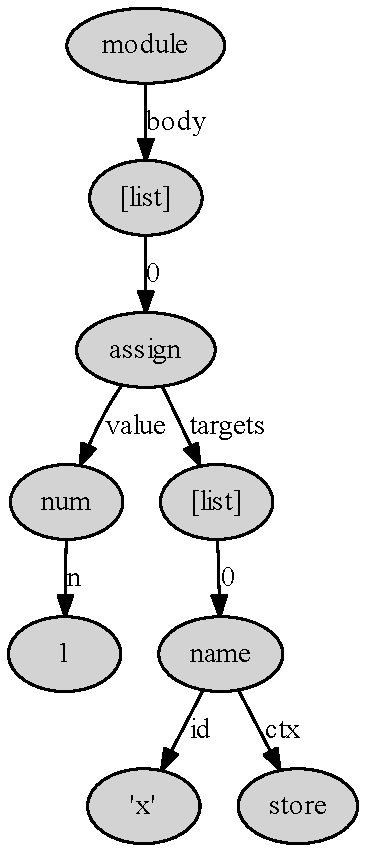
\includegraphics[scale=0.7]{figures/simple_ast.pdf}
    \caption{The syntax tree of the code in \cref{ast_code}}
  \end{subfigure}
  
  \caption{A piece of code and the corresponding syntax tree}
  \label{ast_example}
\end{figure}
